\section{Syllogistique}

	



%
%\begin{frame}
%	\titre{Notions de base}
% 
%	\begin{description}[labelindent=6pt,style=multiline,leftmargin=1.3in]
%		 \setlength\itemsep{1.4em}
%
%		\item[Raisonnement] Le raisonnement \pause
%		\item[Sens] L'expression formelle des hypothèses et conclusions\pause
%		\item[] Cette façon de s'exprimer forme un langage\pause
%		\item[Langage] Les correspondances entre ce langage et celui du quotidien, dit naturel
%
%
%	\end{description}
%
%
%\end{frame}

%
%\begin{frame}
%	\titre{Notions de base}
%	
%	\begin{description}[labelindent=6pt,style=multiline,leftmargin=1.3in]
%		 \setlength\itemsep{1.4em}
%
%		\item[Logique] \only<1>{?} \only<2>{Etude du raisonnement ?} \only<3->{Etude des \textbf{inférences}} \pause \pause
%\pause
%		\item[Inférence]  Dériver une \textbf{conclusion} à partir de \textbf{prémisses} vraies \pause ou supposées vraies \pause
%
%		\item[] Processus naturel et psychologique \pause
%		\item[] mais pas l'objet d'étude des logiciens (et linguistes) \pause
%		\item[Plutôt] la façon dont \textbf{s'expriment} les raisonnements \pause : on va s'intéresser à leur \textbf{forme}.
%
%
%	\end{description}
%
%
%\end{frame}

%
%\begin{frame}
%	\titre{Notions de base}
%	
%	\begin{description}[labelindent=6pt,style=multiline,leftmargin=1.3in]
%		 \setlength\itemsep{1.4em}
%
%		\item[Logique] Etude des propriétés formelles des inférences correctes \pause
%		\item[]
%
%	\end{description}
%
%
%\end{frame}


\begin{frame}
	\titre{Notions de base : inférence}
	
	\begin{description}[labelindent=6pt,style=multiline,leftmargin=1.3in]
		 \setlength\itemsep{1.4em}	

		\item[définition] Dérivation une \textbf{conclusion} à partir de \textbf{prémisses} vraies \pause ou supposées vraies \pause

	\item[Remarque] Un raisonnement est une ou plusieurs inférences imbriquées
	
	\end{description}
\end{frame}


\begin{frame}
	\titre{Notions de base : syllogisme}
	
	\begin{description}[labelindent=6pt,style=multiline,leftmargin=1.3in]
		 \setlength\itemsep{1.4em}


		\item[définition] Mise en forme d'une inférence\pause

	\item[Exemples] 
\begin{tabular}{l}
Je pense\\\hline Je suis\\ 
\end{tabular}

\pause
\item[] \begin{tabular}{l}
Tous les canards boitent\\José est un canard\\\hline José boite\\ 
\end{tabular}

\pause
%\item[] \begin{tabular}{l}
%Tous les hommes sont mortels\\Les mortes sont désespérés\\Les désespérés font des bêtises\\Rouler sans permis est une bêtise\\\hline Il y a des hommes qui roulent sans permis\\ 
%\end{tabular}
\item[] \begin{tabular}{l}
Nulle chaise ne respire\\Tout Homme respire\\\hline Aucun Homme n'est une chaise\\ 
\end{tabular}

	\end{description}

\end{frame}



\begin{frame}
	\titre{Notions de base : syllogistique}
	\only<1>{Etude des syllogismes}
%\pause
	%\only<2>{\includegraphics[scale=0.083]{silog.JPG}}
	
\end{frame}

\begin{frame}
	\titre{Notions de base : application}
	
\begin{tabular}{lr}
Tous les canards boitent & \hspace{2cm} prémisse numéro 1 \\
José est un canard & prémisse numéro 2 \\ \cline{1-1}
 José boite & conclusion\\ \\ \\
\end{tabular}

\pause

Ce syllogisme vous semble-t'il \textit{raisonnable} ? \pause \newline 

Normalement oui \pause : on va du général au spécifique% en \textit{appliquant} la première prémisse avec José, ce qu'on a le droit de faire grâce à la deuxième \newline \pause

%Analogie avec, par exemple, $f(x) = 3\times x + 2$, donc $f(5) = 17$

%
%\begin{description}[labelindent=6pt,style=multiline,leftmargin=1.3in]
%		 \setlength\itemsep{1.4em}
%
%
%		\item[Attention] On ne met pas n'importe quoi en prémisse ou conclusion \pause
%		\item[] On met des \textbf{propositions} \pause
%		\item[] Une expression qu'on peut considérer comme \textbf{vraie} ou \textbf{fausse}
%
%
%	\end{description}

\end{frame}



\begin{frame}
	\titre{Notions de base : application bis}
	
\begin{tabular}{lr}
Tous les canards boitent & \hspace{2cm} prémisse numéro 1 \\ \cline{1-1}
 Jean-Michel boite & conclusion\\ \\ \\
\end{tabular}

\pause

Ce syllogisme vous semble-t'il \textit{raisonnable} ? \pause \newline 

Normalement non \pause : la prémisse 1 est un \textit{contrat} : si tu me \textit{garantis} qu'un objet $x$ est un \textit{canard}, je te garantis qu'il boite.\newline \pause

Il nous manque ici l'information, assertée par une prémisse, que Jean-Michel est un canard \pause \newline

%C'est comme avoir $f(x) = 3\times x + 2$ et essayer de calculer $f(patate)$ \pause \newline

Analogie avec les types en programmation ($int \rightarrow int$)

\end{frame}


\begin{frame}
	\titre{Notions de base : exclusivité}
	%TODO : rajouter une slide pour discuter de ce que recouvre ou non `Homme'
	%ie. vivant ou non (définition précise des termes, tout ça tout ça)
\begin{tabular}{lr}
Aucune chaise ne respire& \hspace{1cm} prémisse numéro 1 \\ 
Tout être humain respire & prémisse numéro 2 \\ \cline{1-1}
Aucun être humain n'est une chaise & conclusion\\ \\ \\
\end{tabular}

\pause

Ce syllogisme vous semble-t'il \textit{raisonnable} ? \pause \newline 

Normalement oui \pause : la prémisse 1 dit qu'être une chaise et respirer sont deux propriétés incompatibles (ou mutuellement exclusives)\newline \pause

La prémisse 2 dit que les Hommes respirent, et donc qu'ils ont `fait leur choix` entre les deux propriétés

\end{frame}


\begin{frame}
	\titre{Notions de base : validité vs. vérité}
	
\begin{tabular}{lr}
Aucun enfant ne respire& \hspace{1cm} prémisse numéro 1 \\ 
Tout être humain respire & prémisse numéro 2 \\ \cline{1-1}
Aucun être humain n'est un enfant& conclusion\\ \\ \\
\end{tabular}

\pause

Ce syllogisme vous semble-t'il \only<2-6>{\textit{raisonnable}} \only<7>{\textbf{valide}} ? \pause \newline 

Normalement oui \pause : au niveau du raisonnement, c'est complètement équivalent (ou isomorphe) à l'exemple précédent \newline \pause

On suppose \textbf{toujours} les prémisses vraies\newline \pause

`Dans un monde où toutes les prémisses sont vraies, puis-je affirmer de façon raisonnable la conclusion ? ` \pause

\end{frame}


\begin{frame}
	\titre{Notions de base : rigueur}
	
\begin{tabular}{lr}
L'immense majorité des canards boite & \hspace{1cm} prémisse numéro 1 \\ 
Jean-Claude est un canard & prémisse numéro 2 \\ \cline{1-1}
Jean-Claude boite & conclusion\\ \\ \\
\end{tabular}

\pause

Ce syllogisme vous semble-t'il \textbf{valide} ? \pause \newline 

Normalement non \pause : on doit toujours \textit{chercher la petite bête}\newline \pause

`Dans un monde où l'ensemble des prémisses est vrai, puis-je affirmer \only<5>{de façon raisonnable} \only<6->{\textbf{de façon \underline{certaine}}} la conclusion ? ` \newline \pause \pause 

La logique, c'est (aussi) l'art d'être chiant

\end{frame}


\begin{frame}
	\titre{Notions de base : abstraction}
	
\begin{tabular}{lr}
Je pense & \hspace{2cm} prémisse numéro 1 \\ \cline{1-1}
 Je suis & conclusion\\ \\ \\
\end{tabular}

\pause

Ce syllogisme vous semble-t'il \textbf{valide} ? \pause \newline 

Normalement non \pause : aucun lien formel entre la prémisse et la conclusion\newline \pause

On va chercher un système \textbf{abstrait} \pause et \textbf{minimal} (voire fini)  \newline \pause

\only<1-6>{\begin{tabular}{l}
\textcolor{white}{Tous les canards boitent}\\\textcolor{white}{José est un canard}\\\textcolor{white}{José boite}\\ 
\end{tabular}}
\only<7>{\begin{tabular}{l}
Tous les canards boitent\\José est un canard\\\hline José boite\\ 
\end{tabular}}
\pause
\only<8>{\begin{tabular}{l}
Tous les canards ont la propriété de boiter\\José est un canard\\\hline José a la propriété de boiter\\ 
\end{tabular}}
\pause
\only<9>{\begin{tabular}{l}
Tous les X ont la propriété Y\\
Z est un X\\ \cline{1-1}
Z a la propriété Y\\
\end{tabular}}
\end{frame}

% ajouts sur l'abstraction
% -----------------------------------


\begin{frame}
	\titre{Notions de base : abstraction}
	
Cette recherche d'abstraction est le prolongement naturel de la distinction qu'on a faite entre \textbf{vérité} (dont on se fiche) et \textbf{validité} (qu'on cherche à \textit{formaliser}, c'est à dire qu'on veut décrire intégralement à l'aide d'un ensemble fini de règles) \pause \newline 

L'idée, c'est d'avoir des principes \textbf{généraux}, qui marcheront même dans le plus bizarre des mondes, puis de les appliquer à (ou instancier avec) un monde en particulier qui contiendra plein de règles comme \newline `ne pas valider LL $\rightarrow$ ne pas valider son année` \pause \newline 

Cette phrase n'est pas très chouette, peut-on la reformuler de façon \textbf{équivalente} mais moins négative ?

\end{frame}

\begin{frame}
	\titre{Notions de base : abstraction}
	
L'idée que les \textit{règles particulières} de \textbf{notre} monde sont à distinguer de certaines règles plus fondamentales, ou universelles, préfigure le \textbf{générativisme}. \newline \pause

La linguistique générative est une théorie portée par Noam Chomsky (et ses camarades) à partir des années 50 qui postule une structure commune à toutes les langues. \newline \pause

Intuitivement, il existe (selon eux) une langue abstraite qui contient par exemple la notion de sujet / verbe / complément qui est ensuite \textit{instanciée} en français, anglais, coréen, turque etc... avec à chaque fois différents paramètres (vocabulaire, ordre SVO etc...)


\end{frame}


\begin{frame}
	\titre{Notions de base : abstraction}
	\pause
Une analogie expérimentale : \pause Fortnite vs. PUBG \newline \pause
	
Les deux jeux, ainsi que les $1329$ autres du genre, diffèrent dans leurs directions artistiques, armes, \textit{maps} etc\pause, mais ces différences sont transcendées par un ADN de base, ou le genre donc, c'est à dire les grands principes (Une île, 100 clampins, une zone qui se réduit, etc) \newline \pause

On peut séparer les `grandes règles`, qui distinguent le \textit{Battle royale} d'autres genre de jeux, des spécificités de chaque BR qui les distinguent les uns des autres. \newline \pause

Même différence entre l'étude des \textbf{langues} \pause et du \textbf{langage}

\end{frame}



\begin{frame}
	\titre{Notions de base : abstraction}

En effet, la communication repose sur une longue \textit{chaine de production}, qui part de l'idée abstraite qu'on veut exprimer et débouche sur une suite de sons (si on est à l'oral).\pause \newline

En gros, on construit d'abord le \textit{sens} précis de l'idée (c'est la \textbf{sémantique}), on traduit ce sens en structure de phrase (c'est la \textbf{syntaxe}), on calcule la suite de sons qui correspond à cette phrase (c'est la \textbf{phonologie}) et on effectue les mouvements articulatoires correspondant (c'est la \textbf{phonétique}).\newline


\end{frame}

\begin{frame}
	\titre{Notions de base : abstraction}

C'est une vision extrêmement simplifiée, mais qui permet d'entrevoir la diversité des processus en jeu pour simplement parler.\pause \newline

Chaque processus étant en soi extrêmement complexe, il est raisonnable de les étudier séparément. Par exemple, le raisonnement fait partie du \textit{sens} \pause(même si on peut l'observer - notamment - via la syntaxe !).\pause \newline

Clairement, la syntaxe et (surtout) la phonétique et la phonologie dépendent de la langue utilisée, mais est-ce le cas de la sémantique ?


\end{frame}



\begin{frame}
	\titre{Notions de base : abstraction}

Ca rejoint l'Hypothèse de Sapir-Whorf\footnote{dont vous avez peut-être entendu parler dans l'excellent film `Premier contact` / `\textit{Arrival}`}, selon laquelle notre vision du monde dépend directement de notre langue. \pause \newline

La question n'est évidemment pas résolue (ni très clairement posée). \pause \newline

Voir cependant le cas très particulier du Pirahã, et de sa relation avec le générativisme et Sapir-Whorf (\textcolor{blue}{\href{http://cpc.cx/khG}{ici}} pour commencer).

\end{frame}

\begin{frame}
	\titre{Notions de base : abstraction}
\only<1->{\textcolor{white}{Olala ligne cachée} \newline}
BREF \pause \newline
	
En syllogistique, tous les mots pas \textit{fonctionnels} (tout ce qui n'est pas `tout`, `aucun`, `est`, `ne pas` etc) sont à considérer comme des variables. \newline 


\only<1-2>{
\textcolor{white}{\begin{tabular}{l}
Tout ce qui est rare est cher\\José arrose la route\\\hline La route est mouillée\\ 
\end{tabular}}
\textcolor{white}{discret saut à la ligne}\newline

\textcolor{white}{Ca, c'est ok du point de vue de la syllogistique parce qu'on considère `être bon marché` et `être rare` comme deux propriétés lambdas}
}

\pause
\only<3>{\begin{tabular}{l}
\textcolor{white}{Tout ce qui est rare est cher}\\\textcolor{black}{José arrose la route}\\\hline \textcolor{black}{La route est mouillée}\\ 
\end{tabular}
\textcolor{white}{discret saut à la ligne}\newline

\textcolor{white}{Ca, c'est ok du point de vue de la syllogistique parce qu'on considère `être bon marché` et `être rare` comme deux propriétés lambdas}
}

\pause
\only<4>{\begin{tabular}{l}
\textcolor{white}{Tout ce qui est rare est cher}\\X effectue l'action Y sur Z\\\hline Z est R\\ 
\end{tabular}
\textcolor{white}{discret saut à la ligne} \newline

\textcolor{white}{Ca, c'est ok du point de vue de la syllogistique parce qu'on considère `être bon marché` et `être rare` comme deux propriétés lambdas}
}


\pause
\only<5->{
\begin{tabular}{l}
Tout ce qui est rare est cher\\Un cheval bon marché est rare\\\hline Un cheval bon marché est cher\\ 
\end{tabular}
\pause
\textcolor{white}{discret saut à la ligne} \newline

Ca, c'est ok du point de vue de la syllogistique parce qu'on considère `être bon marché` et `être rare` comme deux propriétés lambdas
}

\end{frame}


% -----------------------------------

	
\begin{frame}
	\titre{Ingrédients}
	
	\begin{description}[labelindent=6pt,style=multiline,leftmargin=1.3in]
		 \setlength\itemsep{1.4em}
\pause
\item[Hein ?] On n'a pas caractérisé ce qu'on peut utiliser comme prémisse ou conclusion
\pause
\item[Exemple] \begin{tabular}{l}
Je\\
On mange à quelle heure ?\\ \cline{1-1}
serveur blond\\
\end{tabular}
\pause \newline
\item[Idée] On ne veut utiliser que des énoncés qui contiennent du sens 

\pause
\item[] C'est ce qu'on va appeler les \textbf{propositions}
	\end{description}
\end{frame}



\begin{frame}
	\titre{Proposition}
	
	\begin{description}[labelindent=6pt,style=multiline,leftmargin=1.3in]
		 \setlength\itemsep{1.4em}

\item[Intuitivement] Une expression que l'on peut considérer comme \textbf{vraie} ou \textbf{fausse}
\pause
\item[Techniquement] Une expression qui peut recevoir une \textbf{valeur de vérité} 
\pause
\item[Exemples] Il pleut \pause
%\item[] Jean-Paul a faim et Jean-Charles a soif \pause 
\item[] Si vous faites les exos hebdomadaires, vous aurez un bonus sur votre note finale \pause
%\item[] Brian de Palma est un réalisateur génial \pause
\end{description}
 Les hommes justes qui redoutent la puissance de Dieu n’endureront pas les
souffrances éternelles de l’enfer.
\end{frame}


\begin{frame}
	\titre{Les \textbf{non-}propositions}
	
	\begin{description}[labelindent=6pt,style=multiline,leftmargin=1.3in]
		 \setlength\itemsep{1.4em}

\item[`Petites` expressions] Je (référence)
\pause
\item[] Grand (prédicat) \pause
\item[] Actrice norvégienne (prédicat complexe) \pause
\item[] Manger bruyamment (id) \pause
\item[Interrogatives] A quelle heure on mange ? \pause
\item[Impératives] Ne me parle pas de Jean-Louis 
\end{description}
\end{frame}



\begin{frame}
	\titre{Classification des props.}
	Propositions complexes vs. simples \newline
	\pause
	
	\begin{description}[labelindent=6pt,style=multiline,leftmargin=1.3in]
		 \setlength\itemsep{1.4em}

\item[Complexe] contient d'autres propositions \pause
\item[Exemples] Jean-Charles a faim et Jean-Luc a soif\pause
\item[] Chloé est triste car son amie l'a abandonnée\pause
\item[Attention] Une prop. complexe ne \textit{porte} pas forcément \textbf{le sens} d'autres propositions \pause
\item[Exemple] Si je me réveille demain, j'irai en cours
%\item[Remarque] \only<7>{Brian de Palma est un réalisateur américain} \only<8>{Jules est un faux blond} \pause
\end{description}
\end{frame}


\begin{frame}
	\titre{Classification des props.}
	Propositions complexes vs. simples \newline

	
	\begin{description}[labelindent=6pt,style=multiline,leftmargin=1.3in]
		 \setlength\itemsep{1.4em}

\item[Remarque] Les props. complexes peuvent être piégeuses\footnote{Notamment vis-à-vis de la généralisation, ou systématisation, dont on a discuté la dernière fois}\pause
\item[Exemple] Brian de Palma est un réalisateur américain \pause
\newline $\Rightarrow$ Brian de Palma est américain \pause
\newline $\Rightarrow$ Brian de Palma est un réalisateur\pause
\item[vs.] Jules est un faux blond \pause
\newline $\not\Rightarrow$ Jules est blond \pause
\newline $\not\Rightarrow$ Jules est faux (??)

\end{description}
\end{frame}



\begin{frame}
	\titre{Classification des props.}
	Propositions complexes vs. simples \newline

	
	\begin{description}[labelindent=6pt,style=multiline,leftmargin=1.3in]
		 \setlength\itemsep{1.4em}

\item[Remarque] Une prop. peut être arbitrairement complexe \pause
% expliquer que la littérature est pas entièrement claire, mais à priori approche algèbrique
% de toute façon, OSEF au fond de Port-Royal, autant prendre des bons refléxes pour après
% dessin avec un simili-arbre-syntaxique
\item[Exemple] Si Alice apprend que Bob a dit à Charles que Diane en veut à Elsa parce qu'elle a dit du mal du dessin que Flavien lui a fait quand Georges est venu à l'anniversaire d'Hector, Inès sera triste. \pause
\item[Props. simples] Du coup, les propositions \textit{atomiques}

\end{description}
\end{frame}



\begin{frame}
\titre{Retour sur l'exemple}

La notion \underline{précise} de prop. complexe est très boiteuse (et on va d'ailleurs très vite s'en désintéresser)\newline \pause

La définition donnée est \textbf{externe}, dans le sens où elle nous aide à \textit{reconnaître} des propositions (trouvées n'importe où)\pause \newline

On trouve aussi dans la littérature une définition \textbf{interne}, c'est à dire qui décrit la \textit{construction} des propositions complexes, mais elle n'est pas très formelle (donc pas super satisfaisante).\newline \pause

En logique propositionnelle et du premier ordre, on aura une définition interne bien définie et carrée, qui du coup sera dure à appliquer en pratique (compromis auquel on aura du mal à échapper).

\end{frame}

%
%\begin{frame}
%	\titre{Retour sur l'exemple}
%	
%`Sous-propositions` de l'exemple
%	
%\begin{description}[labelindent=6pt,style=multiline,leftmargin=4in]
%\item[Inès sera triste]
%\end{description}
%
%\begin{description}[labelindent=6pt,style=multiline,leftmargin=4in]
%\item[Alice apprend que (...) à l'anniversaire d'Hector]
%\end{description}
%
%
%\begin{description}[labelindent=6pt,style=multiline,leftmargin=4in]
%\item[Bob a dit (...) à l'anniversaire d'Hector]
%\end{description}
%
%
%\begin{description}[labelindent=6pt,style=multiline,leftmargin=4in]
%\item[Diane en veut à (...) à l'anniversaire d'Hector]
%\end{description}
%
%\begin{description}[labelindent=6pt,style=multiline,leftmargin=4in]
%\item[Diane en veut à Elsa]
%\end{description}
%
%\begin{description}[labelindent=6pt,style=multiline,leftmargin=4in]
%\item[Elsa a dit du mal du dessin que Flavien lui a fait quand Georges est venu à l'anniversaire d'Hector]
%\end{description}
%
%
%\end{frame}
%
%
%\begin{frame}
%	\titre{Retour sur l'exemple}
%	
%\begin{description}[labelindent=6pt,style=multiline,leftmargin=4in]
%\item[Alice apprend]
%\end{description}
%\pause NON\pause, plusieurs versions du verbe `apprendre`\pause : `X apprend`\pause, `X apprend Y`\pause, `X apprend Y à Z`\pause, etc ?\pause
%
%
%\begin{description}[labelindent=6pt,style=multiline,leftmargin=4in]
%\item[Diane a dit du mal du dessin]
%\end{description}
%\pause NON\pause, sans le `que truc`, `le dessin` ne désigne plus (forcément) le même objet\pause, on a donc une proposition qui n'apparaît pas dans la phrase complète
%\pause
%\begin{description}[labelindent=6pt,style=multiline,leftmargin=4in]
%\item[Elsa a dit du mal]
%\end{description}
%\pause NON\pause, même raison\pause : en enlevant `du dessin`, on change complètement de proposition
%
%
%\end{frame}
%
%
%\begin{frame}
%	\titre{Retour sur l'exemple}
%	
%\begin{description}[labelindent=6pt,style=multiline,leftmargin=4in]
%\item[Flavien a fait un dessin à Diane quand Georges est venu à l'anniversaire d'Hector]
%\end{description} 
%\textcolor{white}{\_} \newline
%\begin{description}[labelindent=6pt,style=multiline,leftmargin=4in]
%\item[Georges est venu à l'anniversaire d'Hector]
%\end{description}
%\pause
%\begin{description}[labelindent=6pt,style=multiline,leftmargin=4in]
%\item[?]
%\end{description}
%
%\end{frame}
%
%
%\begin{frame}
%		\titre{Retour sur l'exemple}
%%	Si Alice apprend que Bob a dit à Charles que Diane en veut à Elsa parce qu'elle a dit du mal du dessin que Flavien lui a fait quand Georges est venu à l'anniversaire d'Hector, Inès sera triste. 
%	
%	\begin{tikzpicture}[scale=.53]
%
%\Tree[.{si \_ alors \_} [.{\_ apprend \_} Alice [.{\_ a dit \_ à \_} Bob [.{\_ parce que \_ } {Diane en veut à Elsa$_1$} [.{\_ a dit \_} elle$_1$ [.{du \_ de \_} mal [.{le \_ que \_ } dessin [.{\_ quand \_} {Flavien lui a fait} {\begin{tabular}{c}
%     Georges est venu  \\
%     à l'anniversaire d'Hector \\
%  \end{tabular}} ] ] ] ] ] Charles ] ] {Inés sera triste} ]
%\end{tikzpicture}
%
%	
%	\end{frame}


\begin{frame}
	\titre{Classification des props.}
	Propositions (simples) \textbf{catégoriques} vs. \textbf{thétiques} \newline
	
		\begin{description}[labelindent=6pt,style=multiline,leftmargin=1.3in]
		 \setlength\itemsep{1em}
\pause
\item[Def. classique] Une propostion est une expression comportant un sujet et un prédicat (une propriété)
\pause
\item[Exemple] \underline{Le petit chat} est \underline{mort}
\pause 
\item[] \underline{Jean-Louis} est un \underline{canard}
		 \item[] \textcolor{white}{ligne cachée}
		 \item[] \textcolor{white}{ligne cachée}

	\end{description}
\end{frame}


\begin{frame}
	\titre{Classification des props.}
	Propositions (simples) \textbf{catégoriques} vs. \textbf{thétiques} \newline
	
		\begin{description}[labelindent=6pt,style=multiline,leftmargin=1.3in]
		 \setlength\itemsep{1em}
\item[Sujet] Expression référentielle designant un individu (une entité $\in \cal U$) ou une classe d'indivus/entités \pause
\item[] $\Rightarrow$ \textbf{Ce dont on parle}\pause
\item[Prédicat] Propriété que l'on affirme de / que l'on attribue à un sujet \pause
\item[] Techniquement, c'est une fonction de vérité $\cal U \rightarrow \{V,F\}$ \pause
\item[] $\Rightarrow$ \textbf{Ce qu'on en dit}

	\end{description}
\end{frame}


\begin{frame}
	\titre{Classification des props.}
	Propositions (simples) \textbf{catégoriques} vs. \textbf{thétiques} \newline
	
		\begin{description}[labelindent=6pt,style=multiline,leftmargin=1.3in]
		 \setlength\itemsep{1em}
\item[Définition] Les propositions qui obéissent clairement à cette décomposition sont appelées (depuis Aristote) \textbf{jugements catégoriques} \pause
\item[Par contraste] les \textbf{jugements  thétiques} n'ont pas de sujet \textit{réel}\pause, même s'il peut y avoir un sujet grammatical \pause
\item[] Il faisait beau 
\item[] Il y a des fleurs
	\end{description}
\end{frame}



\begin{frame}
	\titre{Classification des props.}
	Propositions (simples) \textbf{catégoriques} vs. \textbf{thétiques} \newline
	
La notion est importante en syllogistique (on y revient), mais plus tard critiquée, notamment par Frege \pause \newline

De façon générale, les classes des propositions en syllogistiques sont peu élégantes et pas toujours très bien définies\pause \newline

Les formalismes plus mathématiques \textit{à la Frege} (ie. la logique propositionnelle) s'attaqueront à ce problème\pause \newline

Aujourd'hui, il est évident que la distinction props. catégoriques / thétiques est pas claire

\end{frame}



\begin{frame}
	\titre{Classification des props.}
	Propositions (simples et catégoriques) \textbf{singulières} vs. \textbf{quantifiées}\newline
	
		\begin{description}[labelindent=6pt,style=multiline,leftmargin=1.3in]
		 \setlength\itemsep{1em}
\item[Singulières] Les phrases ayant un sujet référentiel simple, \textbf{unique} et \textbf{identifié}\pause
\item[Exemple] Lapinot est gentil \pause
\item[] Mon voisin d'en face est photographe \pause
\item[] Le petit chat n'est (finalement) pas mort \pause
\item[] J'ai mal dormi
	\end{description}
\end{frame}

\begin{frame}
	\titre{Classification des props.}
	Propositions (simples et catégoriques) \textbf{singulières} vs. \textbf{quantifiées}\newline
	
		\begin{description}[labelindent=6pt,style=multiline,leftmargin=1.3in]
		 \setlength\itemsep{1em}
\item[Quantifiées] Sujet collectif \pause
\item[Exemple] Tous les élèves m'écoutent \pause
\item[] Quelques films magnifiques sont sortis cette année \pause
\item[] Personne n'a rien à cacher\pause
\item[Question] Le dernier exemple n'est pas très joli, est-ce qu'on peut en trouver une autre formulation (équivalente) ?
	\end{description}
\end{frame}


\begin{frame}
	\titre{Classification des props.}
	%Propositions \textbf{singulières} vs. \textbf{quantifiées}
	
		\begin{description}[labelindent=6pt,style=multiline,leftmargin=1.3in]
		 \setlength\itemsep{1em}
\item[Exemple] Personne n'a rien à cacher \pause $\equiv$ Tout le monde a quelque chose à cacher\pause
%\item[Remarque] Si vous avez du mal à le voir, remplacez `n'a rien à cacher` par `n'a rien dans la tête`\pause 
\item[Intuition] Comprendre la phrase comme `Pour toute personne $x$, il est faux que $x$ a \textbf{la propriété de n'avoir rien à cacher}`\pause
\item[$\equiv$]  `Pour toute personne $x$, \textbf{il est faux qu'il n'existe pas} $y$ que $x$ doit cacher`\pause
\item[$\equiv$] `Pour toute personne $x$, il existe $y$ que $x$ doit cacher` \pause $\equiv$ `Tout le monde a quelque chose à cacher`

	\end{description}
\end{frame}

\begin{frame}
	\titre{Classification des props. quantifiées}
	
		\begin{description}[labelindent=6pt,style=multiline,leftmargin=1.3in]
		 \setlength\itemsep{1em}
\item[Idée] On va essayer de raffiner la distinction de proposition quantifiée \pause en fonction de la `nature` de la quantification\pause
\item[Rappel des exemples] Tous les élèves m'écoutent 
\item[] Quelques films magnifiques sont sortis cette année
\item[] Personne n'a rien à cacher\pause
\item[Du coup] des idées ?
	\end{description}
\end{frame}



\begin{frame}
	\titre{Classification des props. quantifiées}
	Propositions \textbf{universelles}
	
		\begin{description}[labelindent=6pt,style=multiline,leftmargin=1.3in]
		 \setlength\itemsep{1em}
\item[En gros] Sujets introduits par `tous les`, `tout`, `chaque` \& cie\only<1-3>{\textcolor{white}{, mais aussi `nul`, `aucun`}}\only<4>{. Autre chose ?\textcolor{white}{oulouloulou}}\only<5->{, mais aussi `nul`, `aucun`}\pause
\item[Exemples] Tous les élèves m'écoutent\pause
\item[] Tout enfant a une friandise préférée\pause
\pause \pause
\item[] Personne n'a rien à cacher \pause
\item[] Nul n'est infaillible\pause
\item[] Aucun linguiste n'est cool
	\end{description}
\end{frame}


\begin{frame}
	\titre{Classification des props. quantifiées}
	Propositions \textbf{universelles}
	
		\begin{description}[labelindent=6pt,style=multiline,leftmargin=1.3in]
		 \setlength\itemsep{1em}
\item[En gros] `tous les`, `tout`, `chaque`, `nul`, `aucun`\pause, encore autre chose ?\pause
\item[Exemples] Un polar coréen, ça finit mal \pause
\item[] Le canard est un mammifère\pause
\item[A rajouter] les phrases introduites par des déterminants non intrinsèquement quantificationnels, mais prenant une valeur universelle\pause
\item[] C'est à dire les généralisations
	\end{description}
\end{frame}


\begin{frame}
	\titre{Classification des props. quantifiées}
	Propositions \textbf{universelles}
	
		\begin{description}[labelindent=6pt,style=multiline,leftmargin=1.3in]
		 \setlength\itemsep{1em}
\item[Intuition] Toute phrase qu'on peut transformer en `Tous les \textit{individus} qui ont la propriété X ont aussi la propriété Y`
\item[Remarque] On peut quantifier sur plusieurs propriétés\pause 
\item[] `Un polar coréen, ça finit mal` $\equiv$ `Tous les individus qui ont la propriété (\textit{complexe}, ou double) d'être des films coréens ont aussi la propriété de finir mal`\pause
\item[Exemple] `Tout film japonais ou pièce allemande classique me fait rire et pleurer`
	\end{description}
\end{frame}

\begin{frame}
	\titre{Classification des props. quantifiées}
	Propositions \textbf{universelles}
	
		\begin{description}[labelindent=6pt,style=multiline,leftmargin=1.3in]
		 \setlength\itemsep{1em}
\item[Exemples ?] Toutes les voitures volent\pause : yes \pause
\item[] Les poules volent \pause : yes \pause
\item[] Tous les allemands n'étaient pas cinéphiles\pause : nein ($\equiv$ `Il y a des allemands qui n'étaient pas cinéphiles`)\pause
\item[] Le joueur moyen de LoL est tendu\pause : yes\pause
\item[] Chaque journée est un enfer\pause : yes\pause
\item[] Tous mes amis ne sont pas fiables\pause : nein
	\end{description}
\end{frame}



\begin{frame}
	\titre{Classification des props. quantifiées}
	Propositions \textbf{particulières}
	
		\begin{description}[labelindent=6pt,style=multiline,leftmargin=1.3in]
		 \setlength\itemsep{1em}
\item[En gros] Propositions introduites par `un`, `certains`, `quelques` \& cie\pause
\item[Exemples] Certains éléphants ont une trompe\pause
\item[] Quelque malheur a dû arriver\pause
\item[] Quelques enfants ont explosé\pause
\item[] Un mec est passé hier soir\pause
\item[] Un poisson a peu de mémoire\pause : ça dépend \pause(mais à priori non)
	\end{description}
\end{frame}


\begin{frame}
	\titre{Classification des props. quantifiées}
	Attention : confusion \textbf{particulières} et \textbf{singulières} 
	
		\begin{description}[labelindent=6pt,style=multiline,leftmargin=1.3in]
		 \setlength\itemsep{1em}
\item[singulière] A propos d'un seul individu \textbf{précis}\pause
\item[Exemples] Jean-Louis a bien mangé\pause
\item[] \textbf{Ce} lapin a de petites oreilles\pause
\item[particulière] Parle d'un individu \textit{pas identifié}\pause
\item[Exemple] \textbf{Un} lapin (quelque part) a de petites oreilles
	\end{description}
\end{frame}

\begin{frame}
	\titre{Classification des props. quantifiées}
	Propositions \textbf{particulières}
	
		\begin{description}[labelindent=6pt,style=multiline,leftmargin=1.3in]
		 \setlength\itemsep{1em}

\item[Remarque] Certains éléphants ont une trompe
\item[] Quelque malheur a dû arriver
\item[] Quelques enfants ont explosé
\item[] Un mec est passé hier soir\pause
\item[Attention] Tous ces énoncés sont vrais s'il y a \textbf{au moins un} élément du sujet qui vérifie le prédicat \pause (désolé, c'est non-négociable)
	\end{description}
\end{frame}


\begin{frame}
	\titre{Classification des props. quantifiées}
	Propositions \textbf{particulières}
	
		\begin{description}[labelindent=6pt,style=multiline,leftmargin=1.3in]
		 \setlength\itemsep{1em}
\item[Rappel] Dans les universelles, on avait des \textbf{quantificateurs} \textbf{affirmatifs} (`tous les`, `tout`, `chaque`, `un`, `le`, etc) et \textbf{négatifs} (`nul`, `aucun`)\pause
\item[Remarque] On a aussi une notion de affirmatif/négatif pour les props particulières\pause, mais qui se fait cette fois au niveau du verbe\pause
\item[Exemples] Certaines banques n'ont pas été braquées
\item[] Au moins un prof n'est pas compétent 
	\end{description}
\end{frame}


\begin{frame}
	\titre{Classification des props. quantifiées}
	On peut donc distinguer 4 classes de propositions quantifiées en faisant intervenir les 2 paramètres \pause
			\begin{description}[labelindent=6pt,style=multiline,leftmargin=1.3in]
		 \setlength\itemsep{1em}
\item[A] Universelle affirmative 
\item[E] Universelle négative
\item[I] Particulière affirmative 
\item[O] Particulière négative\pause
\item[Question] Des trucs qui ont l'air de ne pas aller avec cette classification ?\pause
\item[] Toutes les props. ne sont pas couvertes (`La plupart des X sont Y`)
	\end{description}
	
\end{frame}



\begin{frame}
	\titre{Le dessin pour résumer}
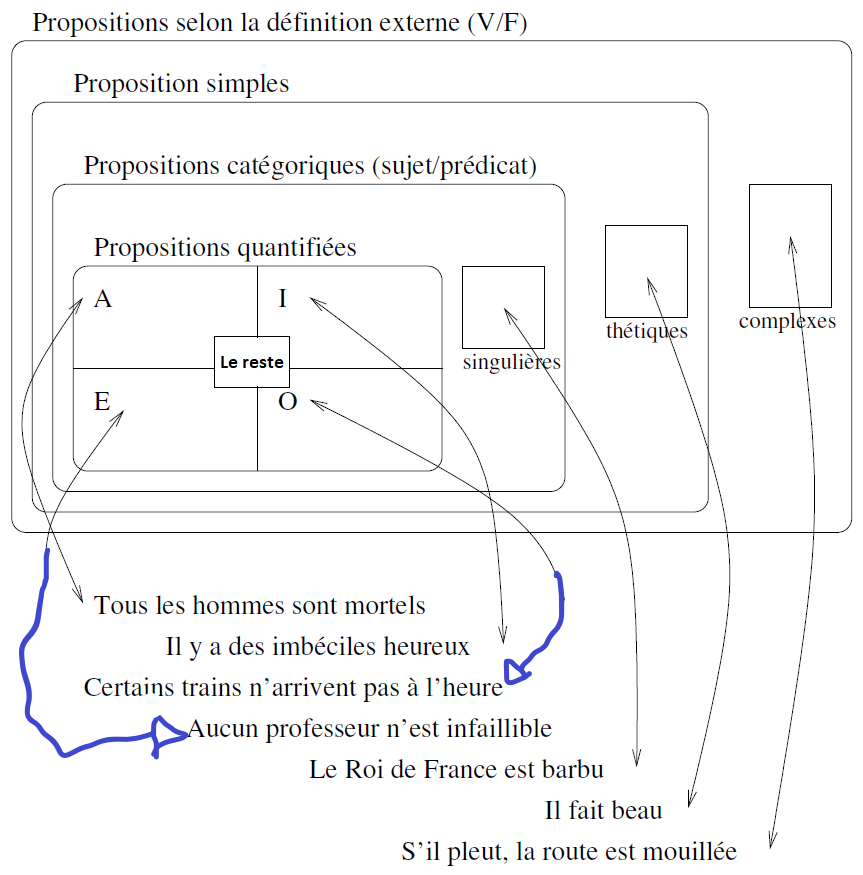
\includegraphics[scale=0.31]{syntheseProps.png}
\end{frame}




%---------------- intro -------------------

\begin{frame}
	\titre{Relations entre propositions}

			\begin{description}[labelindent=6pt,style=multiline,leftmargin=1.3in]
		 \setlength\itemsep{1em}
\item[Inverse \only<5->{?}] \textcolor{white}{lol} 
	 \pause
\item[Exemple] Tout prof est sympa\pause 
\item[] Quelle est la proposition \textit{inverse} ?\pause 
\item[] `Aucun prof n'est sympa` ?\pause 
\item[] Ca dépend de ce qu'on appelle l'\textit{inverse}\pause
\item[] On va distinguer les notions de propositions \textbf{contraires} et \textbf{contradictoires}
	\end{description}
	
\end{frame}



%------------------ Contraire ----------------------
\begin{frame}
	\titre{Relations entre propositions}

			\begin{description}[labelindent=6pt,style=multiline,leftmargin=1.3in]
		 \setlength\itemsep{1em}
\item[Contraires] P et Q sont contraires $\equiv$ elles ne peuvent pas être vraies en même temps 
	 \pause
%\item[En maths] $(P \rightarrow \neg Q) \wedge (Q \rightarrow \neg P)$\pause 
\item[En français] P et Q sont incompatibles\pause 
\item[Exemple] Proposition contraire de `Tout prof est sympa` ?\pause 
\item[] `Aucun prof n'est sympa` ? \pause Oui\pause
\item[] On peut en trouver d'autres ?\pause
\item[] `Il y a au moins un prof qui n'est pas sympa`
	\end{description}
\end{frame}



\begin{frame}
	\titre{Relations entre propositions}

			\begin{description}[labelindent=6pt,style=multiline,leftmargin=1.3in]
		 \setlength\itemsep{1em}
\item[Contraires] P et Q sont incompatibles
	 \pause
%\item[En maths] $(P \rightarrow \neg Q) \wedge (Q \rightarrow \neg P)$\pause 
\item[Exemple] Propositions contraires de `Le chat est mort et le chien est blond` ?\pause 
\item[] Le chat n'est pas mort \pause 
\item[] Le chien n'est pas blond\pause
\item[] Le chat n'est pas mort et le chien n'est pas blond\pause
\item[] Le chat n'est pas mort ou le chien n'est pas blond
	\end{description}
\end{frame}




%------------------------ Contradiction ----------------------------

\begin{frame}
	\titre{Relations entre propositions}

			\begin{description}[labelindent=6pt,style=multiline,leftmargin=1.3in]
		 \setlength\itemsep{1em}
\item[Contradiction] P et Q sont contradictoires si et seulement si elles ne peuvent être ni vraies ni fausses en même temps 
	 \pause
%\item[En maths] $(P \rightarrow \neg Q) \wedge (Q \rightarrow \neg P)$\pause 
\item[En français] On a toujours soit P, soit Q\pause 
\item[Exemple] Proposition contradictoire de `Tout prof est sympa` ?\pause 
\item[] `Il y a au moins un prof qui n'est pas sympa`\pause
\item[] Une autre ? \pause Non, pour toute proposition P, \textbf{unicité} de $\neg P$ (à reformulation près)
	\end{description}
\end{frame}



\begin{frame}
	\titre{Relations entre propositions}

			\begin{description}[labelindent=6pt,style=multiline,leftmargin=1.3in]
		 \setlength\itemsep{1em}
\item[Contradiction] On a toujours soit P, soit Q
	 \pause
%\item[En maths] $(P \rightarrow \neg Q) \wedge (Q \rightarrow \neg P)$\pause 
\item[Exemple] Le chat est mort et le chien est blond\pause 
\item[$\neg$] Le chat n'est pas mort ou le chien n'est pas blond\pause 
\item[Exemple] Certaines baleines sont sympathiques\pause
\item[$\neg$] Aucune baleine est sympathique \pause
\item[Exemple] Certains films français sont pas géniaux \pause
\item[$\neg$] Tous les films français sont géniaux 
	\end{description}
\end{frame}


\begin{frame}
	\titre{Relations entre propositions}

			\begin{description}[labelindent=6pt,style=multiline,leftmargin=1.3in]
		 \setlength\itemsep{1em}
\item[Contradiction] On a toujours soit P, soit Q
	 \pause
%\item[En maths] $(P \rightarrow \neg Q) \wedge (Q \rightarrow \neg P)$\pause 
\item[Exemple] Personne ne comprend ce cours \pause
\item[$\neg$] Quelqu'un comprend ce cours\pause
\item[Question] Vous avez remarqué quelque chose ?\pause
\item[] Quelque chose qui ressemblerait à une règle concernant les contradictions et les propositions quantifiées ?
	\end{description}
\end{frame}


\begin{frame}
	\titre{Relations entre propositions}

			\begin{description}[labelindent=6pt,style=multiline,leftmargin=1.3in]
		 \setlength\itemsep{1em}
\item[A] Tous les profs sont gentils
	 \pause
%\item[En maths] $(P \rightarrow \neg Q) \wedge (Q \rightarrow \neg P)$\pause 
\item[I] Quelques profs sont gentils\pause
\item[E] Aucun prof n'est gentil \pause
\item[O] Quelques profs ne sont pas gentils\pause
\item[Question] Que peut-on dire de chaque couple tiré dans cette liste de propositions ?\pause
\item[Indice] On va devoir introduire deux nouvelles relations (simples) entre propositions
	\end{description}
\end{frame}


\begin{frame}
	\titre{Le carré d'opposition}
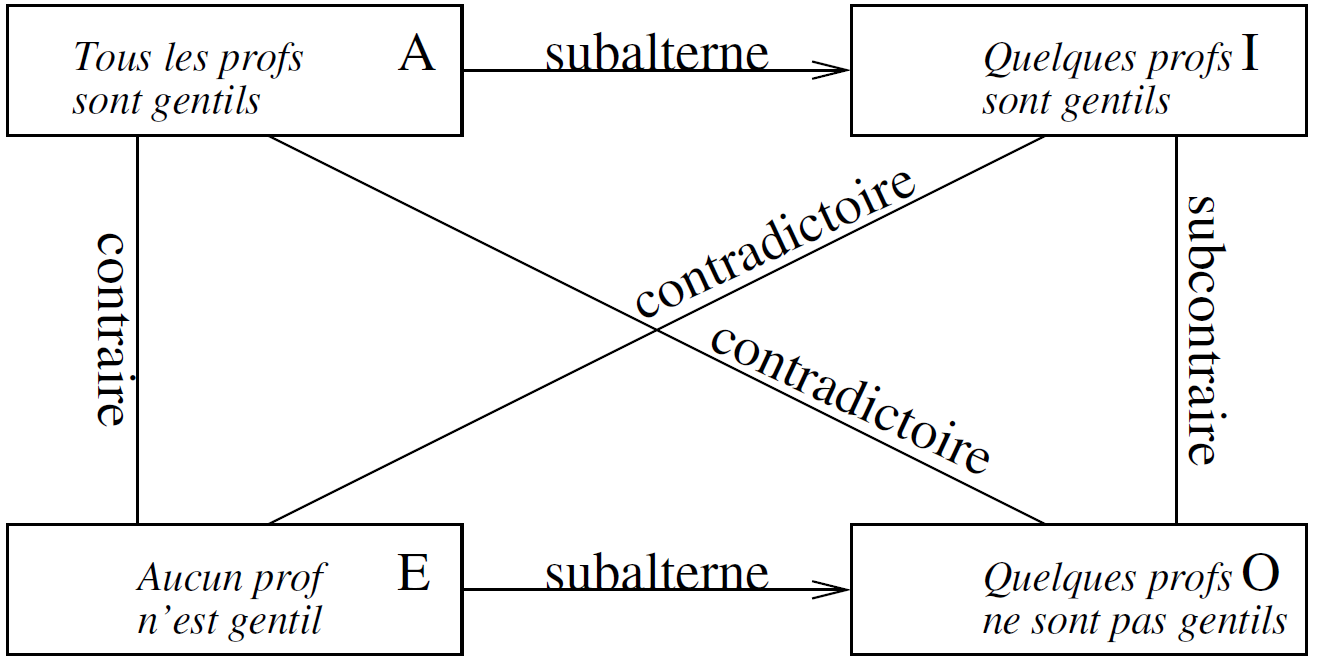
\includegraphics[scale=0.32]{carre.png}
\end{frame}


\begin{frame}
	\titre{Le carré d'opposition}

			\begin{description}[labelindent=6pt,style=multiline,leftmargin=1.3in]
		 \setlength\itemsep{1em}
\item[Subcontraire] P et Q sont subcontraires si elle ne peuvent pas être fausses en même temps\pause
\item[Remarque] I et O sont subcontraires, tandis que leurs contradictions (ou négations) sont contraires entre elles\pause
\item[] Coïncidence ? \pause Sans doute pas\pause
\item[Subalterne] P est subalterne de Q si Q implique P\pause, c'est à dire si chaque fois que Q est vraie, P l'est nécessairement aussi.
	 \pause
\item[def alternative] P est une version appauvrie (en information) de Q
	\end{description}
\end{frame}


\begin{frame}
	\titre{Le début du merdier}
			\begin{description}[labelindent=6pt,style=multiline,leftmargin=1.3in]
		 \setlength\itemsep{1em}
\item[Contraires] P et Q sont contraires $\equiv$ elles ne peuvent pas être vraies en même temps 
\item[Contradiction] On a toujours soit P, soit Q\pause
\item[Cependant] Pour les logiciens ... \pause c'est le contraire !\pause
\item[] Ils ont néanmoins plus l'habitude de dire `propositions inverses` que contraires \pause
\item[] On utilisera $P = \neg Q$ pour `soit P, soit Q` et `P X Q` pour `pas en même temps`
\item[Attention] `P X Q` pas canonique !
	\end{description}
\end{frame}



\begin{frame}
	\titre{Un autre carré bonus}
	
	DM !
%			\begin{description}[labelindent=6pt,style=multiline,leftmargin=1.3in]
%		 \setlength\itemsep{1em}
%\item[Remarque] On dira `R implique S` plutôt que `S est subalterne de R` (vieillot)\pause
%\item[Faits] (P et Q) implique P
%\item[] (P et Q) implique Q\pause
%\item[Explication] On passe de deux infos à une seule d'entre elles, on peut donc parler de perte d'information 
	%\end{description}
\end{frame}

%\begin{frame}
%	\titre{Un autre carré bonus}
%			\begin{description}[labelindent=6pt,style=multiline,leftmargin=1.3in]
%		 \setlength\itemsep{1em}
%\item[Faits] P implique (P ou Q)
%\item[] Q implique (P ou Q)\pause
%\item[Explication] Ici c'est plus fin, mais le même phénomène apparaît : on \textit{brouille} une information autrefois sûre avec une alternative potentielle\pause
%\item[Remarque] On obtient un carré qui permet d'expliquer au sein de la logique comment le `ou` logique inclusif devient exclusif en pratique (cf l'explication en cours)
%	\end{description}
%\end{frame}
%
%


	
\begin{frame}
	\titre{Intro à Port-Royal}
	
	\begin{description}[labelindent=6pt,style=multiline,leftmargin=1.3in]
		 \setlength\itemsep{1.4em}
		 
		 \item[Qui] Antoine Arnauld et Pierre Nicole
		 \pause
		 \item[Où] L'abbaye de Port-Royal (rien à voir avec le métro), haut lieu du jansénisme à l'époque
		 \pause
		 \item[Quand] 1662
		 \pause
		 \item[Quoi] Le bouquin `La logique ou l'art de penser`
		 
	\end{description}
\end{frame}



\begin{frame}
	\titre{Intro à Port-Royal}
	
	\begin{description}[labelindent=6pt,style=multiline,leftmargin=1.3in]
		 \setlength\itemsep{1.4em}
		 
		 \item[But] Distinguer les bons des mauvais syllogismes
		 \pause
		 \item[] C'est à dire ceux qui sont \textbf{valides} et ceux qui ne le sont pas
		 \pause
		 \item[Problème] Y a du travail
		 \pause
		 \item[`Solution`] \textit{Fixer avec précision l'objet d'étude} \pause (cad se resteindre à un chantier plus simple) \pause
		 \item On s'intéresse uniquement aux raisonnements avec 2 prémisses + 1 conclusion\pause, le tout quantifié
 		 
	\end{description}
\end{frame}



\begin{frame}
	\titre{Intro à Port-Royal}
	
	\begin{description}[labelindent=6pt,style=multiline,leftmargin=1.3in]
		 \setlength\itemsep{1em}
		 
		 \item[Rappel] Les \textit{termes} utilisés dans un raisonnement n'ont pas (vraiment) d'importance
		 \pause
		 \item[] \begin{tabular}{l}
Tous les alcooliques sont bigleux\\
Tous les bigleux sont blonds\\ \cline{1-1}
Tous les alcooliques sont blonds\\
\end{tabular}
		 \item[$\equiv$] \begin{tabular}{l}
Tous les barmans sont chauves\\
Tous les chauves sont méchants\\ \cline{1-1}
Tous les barmans sont méchants\\
\end{tabular}\pause


		 \item[$\equiv$] \begin{tabular}{l}
Tous les X sont Y\\
Tous les Y sont Z\\ \cline{1-1}
Tous les X sont Z\\
\end{tabular}
	\end{description}
\end{frame}


\begin{frame}
	\titre{Intro à Port-Royal}
	
	\begin{description}[labelindent=6pt,style=multiline,leftmargin=1.3in]
		 \setlength\itemsep{1em}
		 
		 \item[Idée] On peut donc espérer \textit{énumérer} (lister) l'ensemble des \textbf{schémas} possibles si on trouve les \textbf{paramètres} pertinents
		 \pause
		 \item[Définition] Les conclusions seront de la forme 
\begin{tabular}[t]{clc}
B &est& A\\
\textbf{petit terme} &&\textbf{grand terme}\\
\end{tabular}
 \pause
		 \item[Définition] Pour répondre à la question, on va passer par un autre terme, le \textbf{moyen}
\pause

		 \item[]
\begin{tabular}{cccl}
A  & $\leftrightarrow$ & M & (prémisse) majeure\\
M  & $\leftrightarrow$ & B & (prémisse) mineure\\
\hline
B  & est & A & conclusion\\
\end{tabular}
	\end{description}
\end{frame}


\begin{frame}
	\titre{Figures}
	
	\begin{description}[labelindent=6pt,style=multiline,leftmargin=1.3in]
		 \setlength\itemsep{1em}
		 
		 \item[]
\begin{tabular}{cccl}
A  & $\leftrightarrow$ & M & (prémisse) majeure\\
M  & $\leftrightarrow$ & B & (prémisse) mineure\\
\hline
B  & est & A & conclusion\\
\end{tabular}

\item[Remarque] L'ordre peut changer (d'où les $\leftrightarrow$)\pause, pour un total de 4 combinaisons
\pause
\item[Constantes] A (grand terme) = attribut de la conclusion \pause
\item[] B (petit terme) = sujet de la conclusion \pause 
\item[] M (moyen) = attribut ou sujet \newline \pause 
	\end{description} 

	Majeure (resp. Mineure) = prémisse impliquant le grand (resp. petit) terme 
\end{frame}




\begin{frame}
	\titre{Figures}
	
	\begin{tabular}{ccc}
\begin{tabular}{lcc}
1\iere\ figure	& M & A \\
		& B & M \\
\cline{2-3}
		& B & A \\
\end{tabular}
%

&
\textcolor{white}{lolilol}
&
\begin{tabular}{lcc}
2\ieme\ figure	& A & M \\
		& B & M \\
\cline{2-3}
		& B & A \\
\end{tabular} \\
%


\textcolor{white}{lolilol} & 
\textcolor{white}{lolilol} & 
\textcolor{white}{lolilol} \\


\textcolor{white}{lolilol} & 
\textcolor{white}{lolilol} & 
\textcolor{white}{lolilol} \\


\textcolor{white}{lolilol} & 
\textcolor{white}{lolilol} & 
\textcolor{white}{lolilol} \\

\begin{tabular}{lcc}
3\ieme\ figure	& M & A \\
		& M & B \\
\cline{2-3}
		& B & A \\
\end{tabular}

&
\textcolor{white}{lolilol}
&
\begin{tabular}{lcc}
4\ieme\ figure	& A & M \\
		& M & B \\
\cline{2-3}
		& B & A \\
\end{tabular}
\end{tabular}
\end{frame}



\begin{frame}
	\titre{Modes}
	
	\begin{description}[labelindent=6pt,style=multiline,leftmargin=1.3in]
		 \setlength\itemsep{1em}

\item[Mode] Arrangement de 3 propositions ayant 4 formes possibles (A, I, E ou O) \pause $\rightarrow$ 64 combinaisons (AAA, EIO, AEE, etc ...)\pause
\item[] On va pouvoir combiner figure et mode \pause : si le mode est $Q_1Q_2Q_3$, la grand prémisse sera $Q_1$, la petite sera $Q_2$ et la conclusion sera $Q_3$. \pause
\item[But du jeu] Essayer toutes les figures avec tous les modes \pause pour un total de 256 syllogismes à tester ! 

	\end{description} 
\end{frame}



\begin{frame}
	\titre{C'est parti ! (1/256)}
	
	\begin{description}[labelindent=6pt,style=multiline,leftmargin=1.3in]
		 \setlength\itemsep{1em}

\item[$3^{\grave{e}me}$ figure] \begin{tabular}{cc}
M & A \\
	M & B \\
\cline{1-2}
		B & A \\
\end{tabular}
\item[Mode] AAA \pause
\item[Attention] Les `A` du mode et ceux de la figure n'ont rien à voir ! \pause (personne n'a dit que le formalisme était bien foutu) \pause
\item[Question] Valide ? 

	\end{description} 
\end{frame}



\begin{frame}
	\titre{C'est parti ! (1/256)}
	
	\begin{description}[labelindent=6pt,style=multiline,leftmargin=1.3in]
		 \setlength\itemsep{1em}

\item[Mode + figure] \begin{tabular}{c}
Tous les M sont A\\ 
Tous les M sont B\\ 
\cline{1-1}
Tous les B sont A
\end{tabular} \pause
\item[Explication] On peut imaginer un monde dans lequel il y a uniquement 2 individus, Jean-Michel qui est à la fois M, A et B, et Jean-Charles qui est uniquement B \pause
\item[] Les deux \textbf{hypothèses} sont \textbf{respectées} (tout M est également A et B), mais la \textbf{conclusion} est \textbf{fausse} (JC l'enfreint)\pause
\item[Réponse] Pas valide, car on a un \textbf{contre-exemple} 

	\end{description} 
\end{frame}


\begin{frame}
	\titre{C'est parti ! (1/256)}
	
	\begin{description}[labelindent=6pt,style=multiline,leftmargin=1.3in]
		 \setlength\itemsep{1em}

\item[Mode + figure] \begin{tabular}{c}
Tous les M sont A\\ 
Tous les M sont B\\ 
\cline{1-1}
Tous les B sont A
\end{tabular}
\item[Explication] On peut imaginer un monde dans lequel il y a uniquement 2 individus, Jean-Michel qui est à la fois M, A et B, et Jean-Charles qui est uniquement B
\item[Remarque] Un truc à dire sur ce contre-exemple \only<1>{? \textcolor{white}{pour l'améliorer}}\only<2->{pour l'améliorer ?}\pause  \pause
\item[] Il n'est pas minimal\pause, on peut se passer de Jean-Michel

	\end{description} 
\end{frame}



\begin{frame}
	\titre{Méthodologie}
	
	\begin{description}[labelindent=6pt,style=multiline,leftmargin=1.3in]
		 \setlength\itemsep{1em}
		 
\item[Remarque] \textbf{Un (contre-)exemple sert uniquement à montrer qu'un syllogisme n'est pas valide} \pause
\item[] On pourrait aussi imaginer un monde où il y a un seul individu, qui est M, A et B\pause
\item[] Dans ce cas, hypothèses + conclusion respectées\pause
\item[] Le syllogisme n'en est pas pour autant valide !
\item[] Pour montrer la validité, ça va donc être un peu plus abstrait 
	\end{description} 

	
\end{frame}

\begin{frame}
	\titre{Méthodologie}
	
	\begin{description}[labelindent=6pt,style=multiline,leftmargin=1.3in]
		 \setlength\itemsep{1em}
		 
\item[Par contre] Les contre-exemples se présentent très bien sous la forme de \textbf{diagrammes de Venn} (aussi appelés patatoïdes)\pause
\item[Exemple] 	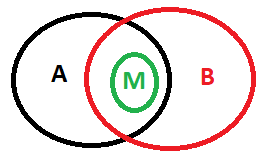
\includegraphics[scale=0.5]{1256.png}\pause
\item[] Chaque \textit{patate} représente l'ensemble des individus qui ont la propriété associée\pause
\item On a bien les hypothèses respectées et la conclusion falsifiée
	\end{description} 

	
\end{frame}







%
%\begin{frame}
%	\titre{C'est parti ! (1/256 prise 2)}
%	
%	\begin{description}[labelindent=6pt,style=multiline,leftmargin=1.3in]
%		 \setlength\itemsep{1em}
% 
%\item[Exemple] 
%\begin{tabular}{c}
%Tous les canards sont mexicains \\
%	Tous les canards jouent au poker \\
%\cline{1-1}
%Tous les joueurs de poker sont mexicains \\
%\end{tabular}
%\pause
%\item[Explication] Soit un monde dans lequel tous les canards sont des joueurs de poker mexicains, et Jean-Luc un joueur de poker non-canard, non-mexicain. Aucune des hypothèses n'est violée, tandis que la conclusion n'est pas vraie. \pause
%\item[Réponse] Pas valide, car on a un \textbf{contre-exemple} 
%	\end{description} 
%\end{frame}
%


\begin{frame}
	\titre{C'est parti ! (2/256)}
	
	\begin{description}[labelindent=6pt,style=multiline,leftmargin=1.3in]
		 \setlength\itemsep{1em}

\item[$1^{\grave{e}re}$ figure] \begin{tabular}{cc}
M & A \\
	B & M \\
\cline{1-2}
		B & A \\
\end{tabular}
\item[Mode] AAA \pause
\item[Question] Valide ? 

	\end{description} 
\end{frame}



\begin{frame}
	\titre{C'est parti ! (2/256)}
	
	\begin{description}[labelindent=6pt,style=multiline,leftmargin=1.3in]
		 \setlength\itemsep{1em}

\item[Mode + figure] \begin{tabular}{c}
Tous les M sont A\\ 
Tous les B sont M\\ 
\cline{1-1}
Tous les B sont A
\end{tabular} \newline
	\end{description}
	
Prenons un B \textbf{arbitraire}\pause, cad sur lequel on n'a aucune autre information \pause
\newline 

La prémisse min. nous dit qu'il est aussi M\pause
\newline

La prémisse maj. nous dit alors qu'il est aussi A\pause \newline

Syllogisme valide \pause : on a montré qu'un individu, \textbf{dont on savait seulement qu'il était B}, est aussi un A. \pause Ca prouve que \textbf{n'importe quel B} sera aussi A

\end{frame}


\begin{frame}
	\titre{C'est parti ! (2/256 prise 2)}
	
	\begin{description}[labelindent=6pt,style=multiline,leftmargin=1.3in]
		 \setlength\itemsep{1em}

\item[Mode + figure] \begin{tabular}{c}
Tous les M sont A\\ 
Tous les B sont M\\ 
\cline{1-1}
Tous les B sont A
\end{tabular} \newline
	\end{description}
	
	 
Prenons un B \textbf{arbitraire}, cad sur lequel on n'a aucune autre information \pause \newline 

La prémisse min. permet de le \textbf{transformer} en M\pause \newline

La prémisse maj. permet de \textbf{transformer} le M obtenu en A \pause \newline

Syllogisme valide \pause : on a montré qu'en \textbf{composant} (combinant) les deux prémisses, on crée \only<1-4>{\textcolor{white}{une \textit{méthode}}}\only<5>{une \textit{méthode}}\only<6>{une \textit{fonction}}\only<7>{un \textbf{programme}} permettant de \textbf{transformer} tout B en A \pause

\end{frame}


%
%\begin{frame}
%	\titre{Méthodo validité}
%	
%Dans le cas d'une démonstration de non-validité d'un syllogisme, vous pouvez utiliser des exemples `concrets` ou rester abstrait, selon ce avec quoi vous êtes le plus à l'aise \newline
%\pause
%
%La non-importance des termes fait que vous pourriez théoriquement avoir le même choix au moment de prouver la validité d'un syllogisme\pause, mais pour vous faire prendre des bonnes habitudes, on va se limiter à l'abstrait \newline
%
%\pause
%En maths, un \textbf{exemple} ne prouve pas un résultat \textit{général}. Ici c'est un cas un peu dégénéré qu'on va donc ignorer.
%
%\end{frame}


\begin{frame}
	\titre{La slide barbante}
	
Vous pouvez choisir d'utiliser le style `$x$ est un A et telle prémisse nous dit que tout A est aussi un M, donc $x$ est un M`\pause, ou `x est un A et telle prémisse permet de \textit{transformer} tout A en M, donc on peut faire de x un M`. \newline \pause

La différence n'est sans doute pas évidente, mais représente les deux (grosses) approches des fondements des mathématiques ! \pause \newline

Le premier style correspond à un point de vue \textbf{théorie des ensembles} (patatoïdes), tandis que la deuxième formulation découle de la \textbf{théorie des types} (programmes). \pause Le schisme entre ces deux théories est une conséquence du \textbf{paradoxe de Russel} (1901$\sim$1903).

\end{frame}



\begin{frame}
	\titre{C'est (re-)parti ! (3/256)}
	
	\begin{description}[labelindent=6pt,style=multiline,leftmargin=1.3in]
		 \setlength\itemsep{1em}

\item[$2^{\grave{e}me}$ figure] \begin{tabular}{cc}
A & M \\
	B & M \\
\cline{1-2}
		B & A \\
\end{tabular}
\item[Mode] AAI \pause
\item[Question] Valide ? 

	\end{description} 
\end{frame}



\begin{frame}
	\titre{C'est (re-)parti ! (3/256)}
	
	\begin{description}[labelindent=6pt,style=multiline,leftmargin=1.3in]
		 \setlength\itemsep{1em}

\item[Mode + figure] \begin{tabular}{c}
Tous les A sont M\\ 
Tous les B sont M\\ 
\cline{1-1}
Certains B sont A
\end{tabular}\pause
\item[Explication] On peut imaginer un monde dans lequel il y a seulement 2 individus : Jean-Michel qui est à la fois A et M, et Jean-Charles qui est uniquement B et M\pause
\item[] Les deux hypothèses sont respectées (tout individu A ou B est également M), mais la conclusion est fausse (le seul B n'est pas A)\pause
\item[Réponse] Pas valide, car on a un \textbf{contre-exemple} 

	\end{description} 
\end{frame}


\begin{frame}
	\titre{C'est (re-)parti ! (3/256 bonus)}
	
	\begin{description}[labelindent=6pt,style=multiline,leftmargin=1.3in]
		 \setlength\itemsep{1em}

\item[AAX + fig. 3] \begin{tabular}{c}
Tous les A sont M\\ 
Tous les B sont M\\ 
\cline{1-1}
[relation entre A et B]
\end{tabular} \pause
\item[Remarque] Etant donnée la figure, aucun mode de la forme AAX ne sera valide
\pause
\item[] En effet, imaginez que M est l'ensemble des individus\pause, alors les deux prémisses deviennent `tous les individus ayant la prop A (ou B) sont des individus`\pause
\item[] Ca n'apporte strictement aucune information, on ne va rien pouvoir conclure

	\end{description} 
\end{frame}






\begin{frame}
	\titre{C'est (re-)parti ! (7/256)}
	
	\begin{description}[labelindent=6pt,style=multiline,leftmargin=1.3in]
		 \setlength\itemsep{1em}

\item[$1^{\grave{e}re}$ figure] \begin{tabular}{cc}
M & A \\
	B & M \\
\cline{1-2}
		B & A \\
\end{tabular}
\item[Mode] III \pause
\item[Question] Valide ? 

	\end{description} 
\end{frame}



\begin{frame}
	\titre{C'est (re-)parti ! (7/256)}
	
	\begin{description}[labelindent=6pt,style=multiline,leftmargin=1.3in]
		 \setlength\itemsep{1em}

\item[Mode + figure] \begin{tabular}{c}
Certains M sont A\\ 
Certains B sont M\\ 
\cline{1-1}
Certains B sont A
\end{tabular}\pause
\end{description}
\only<1>{\vspace{5cm}}
\only<2-3>{
	\begin{description}[labelindent=6pt,style=multiline,leftmargin=1.3in]
		 \setlength\itemsep{1em}
\item[Contre-ex] On a 10 individus $p_1$ à $p_{10}$. $p_1$ est M et A (et pas B), $p_2$ est B et M (et pas A), le reste n'est jamais A et B à la fois\pause
\item[] Les deux hypothèses sont respectées (grâce à $p_1$ et $p_2$), mais la conclusion est fausse (peut se vérifier sur chaque individu)\pause
\end{description}
\vspace{1.47cm}
}

\only<4>{
	\vspace{1.2cm}
	\begin{figure}[H]
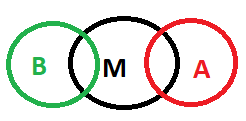
\includegraphics[scale=0.5]{4256.png}
\end{figure}\vspace{1.9cm}}

\pause

\only<5>{
	\vspace{1.2cm}
	\begin{figure}[H]
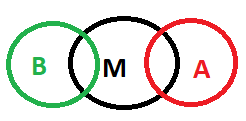
\includegraphics[scale=0.5]{4256.png}
\end{figure}
	\begin{description}[labelindent=6pt,style=multiline,leftmargin=1.3in]
		 \setlength\itemsep{1em}
\item[Réponse] Pas valide, car on a un \textbf{contre-exemple} 
	\vspace{1.1cm}
	\end{description}}

	 
\end{frame}



\begin{frame}
	\titre{C'est (re-)parti ! (7/256)}
	
	\begin{description}[labelindent=6pt,style=multiline,leftmargin=1.3in]
		 \setlength\itemsep{1em}

\item[Mode + figure] \begin{tabular}{c}
Certains M sont A\\ 
Certains B sont M\\ 
\cline{1-1}
Certains B sont A
\end{tabular}
	\end{description} 
De façon générale, on ne pourra jamais rien tirer de deux propositions particulières\pause \newline

Quel que soit le type (A / E / I / O) de la conclusion, on pourra créer une situation qui valide les deux hypotheses (particulières) sans valider la conclusion (comme on vient de le faire)\pause \newline

En fait, pas mal de règles de ce type, qui réduisent l'ensemble des syllogisme à tester, ont été identifiées.


\end{frame}
	


\begin{frame}
	\titre{Règles de base des syllogismes}
	
	\begin{itemize}
	
	\item[1] Le moyen doit être pris au moins une fois universellement\pause
	\item[2]   Les termes de la conclusion ne peuvent point être pris plus universellement dans la conclusion que dans les prémisses\pause
	\item[3]  On ne peut rien conclure de deux propositions négatives\pause
	\item[4]  On ne peut prouver une conclusion négative par deux propositions affirmatives\pause
	\item[5]  La conclusion suit toujours la plus faible partie, cad que s'il y a une des deux propositions négatives, elle est négative, et s'il y en a une particulière, elle doit être particulière\pause
	\item[6]  De deux propositions particulières il ne s'ensuit rien
	
	\end{itemize}
	
\end{frame}
	


\begin{frame}
	\titre{Pause discussion}
	
	\begin{description}[labelindent=6pt,style=multiline,leftmargin=1.3in]
		 \setlength\itemsep{1em}

\item[Remarques] ?\pause
\item[Pts positifs] Différence vérité / validité\pause
\item[] Début de classification ...\pause
\item[Pts négatifs] ... un peu bancale ...\pause
\item[] ... et arbitraire\pause
\item[] Système très \textbf{incomplet} (les propositions valides ne sont pas toutes couvertes) ... \pause
\item[] ... et pourtant redondant (cf A / E / I / O)
\end{description}
\end{frame}
	
	

% 6/256

\begin{frame}
	\titre{C'est (re-)parti ! (?/256)}
	
	\begin{description}[labelindent=6pt,style=multiline,leftmargin=1.3in]
		 \setlength\itemsep{1em}

\item[$4^{\grave{e}me}$ figure] \begin{tabular}{ll}
A & M \\
	M & B \\
\cline{1-2}
		B & A \\
\end{tabular}
\item[Mode] EAO \pause
\item[Question] Valide ? 

	\end{description} 
\end{frame}



\begin{frame}
	\titre{C'est (re-)parti ! (?/256)}
	
	\begin{description}[labelindent=6pt,style=multiline,leftmargin=1.3in]
		 \setlength\itemsep{1em}

\item[Mode + figure] \begin{tabular}{l}
Aucun A n'est M\\ 
Tous les M sont B\\ 
\cline{1-1}
Certains B ne sont pas A
\end{tabular} \newline
	\end{description} \pause
Quand on a une conclusion négative, c'est souvent plus simple de raisonner par l'absurde\pause \newline

On part du principe (potentiellement abusivement ...) que toute propriété est soit fausse, soit vraie.\newline \pause

Si on prouve qu'elle ne peut pas être fausse, elle doit donc forcément être vraie. \pause On va donc supposer qu'elle est fausse, et voir si ça introduit un paradoxe, auquel cas on a gagné.
\end{frame}


\begin{frame}
	\titre{C'est (re-)parti ! (?/256)}
	
	\begin{tabular}{l}
\textcolor{green}{Aucun A n'est M}\\ 
\textcolor{red}{Tous les M sont B}\\ 
\textcolor{blue}{Tous les B sont A}\\ 
\cline{1-1}
[Paradoxe, fin du monde, invasion de sauterelles] \\
\textcolor{white}{lol}
\end{tabular} \newline \pause

\begin{tabular}{cc}
\begin{tabular}{l}
\textcolor{red}{Tous les M sont B}\\ 
\textcolor{blue}{Tous les B sont A}\\ 
\cline{1-1}
\textcolor{purple}{Tous les M sont A}\\
\textcolor{white}{lol}
\end{tabular} 
& \pause \begin{tabular}{l}
\textcolor{purple}{Tous les M sont A}\\
\textcolor{green}{Aucun A n'est M}\\ 
\cline{1-1}
[Paradoxe]\\
\textcolor{white}{lol}
\end{tabular}\end{tabular}\pause
	
En acceptant les deux prémisses originales, `Tous les B sont A` impossible\pause, donc la négation (contradiction) est vraie\pause \newline

On a donc bien `Certains B ne sont pas A`\pause, n'est-ce pas ?

\end{frame}


\begin{frame}
	\titre{Twist}
En fait non, on peut créer un contre-exemple !\pause \newline

Soit un monde dans lequel personne n'est M et où tous les B sont A (puisque c'est un contre-exemple, on choisit)\newline\pause

`Aucun A n'est M` $\Rightarrow$ c'est automatiquement vrai\pause \newline

`Tous les M sont B` $\Rightarrow$ c'est plus étrange, mais c'est vrai aussi : il est vrai que \textbf{chaque} M est aussi un B\pause \newline

 La conclusion `certains B ne sont pas A` est quant à elle fausse. C'est donc bien un contre-exemple

\end{frame}


\begin{frame}
	\titre{Twist}
	
	\begin{description}[labelindent=6pt,style=multiline,leftmargin=1.3in]
		 \setlength\itemsep{1em}
		 \item[Euh, ok ?] Pourquoi ce détour apparemment inutile ?\pause
		 \item[] Étonnement, c'est une `configuration` ($4^{\grave{e}me}$ figure, mode EAO) qui jugée valide dans Port-Royal
		 \end{description}

 \pause	 
	\begin{description}[labelindent=6pt,style=multiline,leftmargin=1.3in]
		 \setlength\itemsep{1em}
		 \item[Alors quoi ?] Une \underline{piste} intéressante à étudier, c'est la notion de \textbf{vérité}
		 %\item[Attention] On étudie la \textbf{validité} des syllogismes, mais la définition utilise celle de la vérité
 	\end{description}
\end{frame}


\begin{frame}
	\titre{Twist}
	
	\begin{description}[labelindent=6pt,style=multiline,leftmargin=1.3in]
		 \setlength\itemsep{1em}
		 \item[Attention] On étudie la \textbf{validité} des syllogismes, mais la définition utilise celle de la vérité\pause
		 \item[] `Dans un monde où les prémisses sont \textbf{vraies}, est-ce qu'on peut assurer que la conclusion sera \textbf{vraie} aussi ? `\pause
		 \item[Question] Dans un monde où personne n'est M, dans quelle mesure est-il vrai que `tous les M sont B` et que `aucun A n'est M` ?\pause
		 \item[Réponse] \textit{Techniquement} c'est vrai, mais \textit{en pratique}, c'est très étrange. \pause Distinction \textbf{sémantique} / \textbf{pragmatique}
 	\end{description}
\end{frame}




\begin{frame}
	\titre{Twist}
	
	\begin{description}[labelindent=6pt,style=multiline,leftmargin=1.3in]
		 \setlength\itemsep{1em}
		 \item[Sémantique] Construction du sens \textit{strict}\pause
		 \item[Pragmatique] Le sens \textit{en pratique}\pause
		 \item[Exemples] Comment le [ou inclusif] logique devient en pratique le [ou exclusif] en pratique \pause
		 \item[] Utilisation de `moins de [un nombre]` \pause
		 \item[] `aucun A n'est M` qui ne passe pas dans un monde où rien n'est M\pause
		 \item[] La linguistique moderne fait bien la distinction entre sémantique et pragmatique, PR non
		 
 	\end{description}
\end{frame}



\begin{frame}
	\titre{Au final}
	
	Liste des syllogismes jugés valides par Port-Royal :
	
	\begin{tabular}{cccc}
	\textcolor{white}{lol} & \textcolor{white}{lol} & \textcolor{white}{lol} & \textcolor{white}{lol} \\
\rm 1\iere\ figure & \rm 2\ieme\ figure & \rm 3\ieme\ figure & \rm 4\ieme\ figure\\
\hline
AAA&AOO&\color{black}AAI&\color{black}AAI\\
\color{black}AII&\color{black}AEE&\color{black}AII&\color{black}AEE\\
\color{black}EAE&\color{black}EAE&\color{black}EAO&\color{black}EAO\\
EIO&EIO&EIO&EIO\\
   &   &\color{black}IAI&\color{black}IAI\\
   &   &OAO&   \\
\end{tabular}


	
\end{frame}





 \begin{frame}
 \titre{Conclusion}
 
 Bon, la logique de Port-Royal c'est pas exactement la formalisation ultime et absolue du raisonnement. \newline \pause
 
Certaines corrections ont été tentées, notamment par Leibniz. \pause Il introduit syllogismes supplémentaires (24 au lieu des 19 de PR), mais les problèmes du formalisme sont trop \textit{profonds}. \pause  \newline

Il introduit aussi des méthodes de \textit{calcul} (preuve) graphiques (patatoïdes (ou diagrammes de Venn), droites de Leibniz), mais rien de très satisfaisant.\pause \newline

Y a quand même des bonnes idées, qu'on va essayer de retrouver sur une base plus solide \pause : \textbf{la logique formelle !}
 
 \end{frame}
 
 
 
 
 
\begin{frame}
	\titre{Exercices - classification}

Diane est cool : \pause proposition singulière (on parle d'une personne clairement identifiée)\pause\newline

Les amis de Diane sont cool : \pause proposition universelle affirmative A (`tout individu ayant la propriété d'être un ami de Diane a aussi la propriété d'être cool`)\pause\newline

Diane et Elsa sont cool : \pause proposition complexe (composée de `Diane est cool` + `Elsa est cool`)\pause\newline

Au moins un ami de Diane n'est pas cool : \pause proposition particulière négative O (Il existe un individu qui a la propriété d'être un ami de Diane mais pas celle d'être cool)

\end{frame}
\begin{frame}
	\titre{Exercices - classification}

Un ami de Diane est cool : \pause proposition particulière affirmative I (Il existe un individu qui a la propriété d'être un ami et celle d'être cool) \pause ... ou universelle affirmative A !\newline\pause

Aucun ami de Diane n'est cool : \pause proposition universelle négative E (Tout individu ayant la propriété d'être un ami de Diane a la propriété de ne pas être cool)\pause\newline

Certains amis de Diane sont cool : \pause proposition particulière affirmative I

\end{frame}
\begin{frame}
	\titre{Exercices - classification}

L'ami pas cool de Diane est moche : \pause proposition singulière \pause (le `le` (abrégé en `l'`) présuppose que la personne mentionnée est clairement identifiée, c'est comme si on utilisait son nom)\pause\newline

Un ami moche de Diane est un bon ami : \pause proposition particulière affirmative I \pause ... ou universelle affirmative A
\end{frame}


\begin{frame}
	\titre{Exercices - négation}

$\neg$(Diane est cool) = \pause Diane n'est pas cool \pause ($\neg$(x est Y) = x n'est pas Y)\pause\newline

$\neg$(Les amis de Diane sont cool) = \pause Au moins un ami de Diane n'est pas cool\pause\newline

$\neg$(Diane et Elsa sont cool) = \pause Diane n'est pas cool ou Elsa n'est pas cool \pause ($\neg (P $ ET $ Q) = \neg P $ OU $ \neg Q$)\pause\newline

$\neg$(Au moins un ami de Diane n'est pas cool) = \pause Tous les amis de Diane sont cool

\end{frame}

\begin{frame}
	\titre{Exercices - négations}
	
	
$\neg$(Un ami de Diane est cool) = \pause Aucun ami de Diane n'est cool (si vous avez répondu I avant) ou Au moins un ami de Diane n'est pas cool (si A)\pause\newline


$\neg$(Aucun ami de Diane n'est cool) = \pause Au moins un ami de Diane est cool\pause\newline

$\neg$(Certains amis de Diane sont cool) = \pause Aucun ami de Diane n'est cool

\end{frame}
\begin{frame}
	\titre{Exercices - négations}
	
	
$\neg$(L'ami pas cool de Diane est moche) = \pause L'ami pas cool de Diane n'est pas moche\pause\newline

$\neg$(Un ami moche de Diane est un bon ami) = \pause Aucun ami de Diane n'est un bon ami (si I), ou Au moins un ami moche de Diane n'est pas un bon ami (si A)

\end{frame}




\begin{frame}
	\titre{Exercices - implications}

`Les amis de Diane sont cool` \appearsAt{2}{black}{$\rightarrow$} `Certains amis de Diane sont cool`\pause\pause\newline

`Aucun ami de Diane n'est cool` \appearsAt{4}{black}{$\rightarrow$} `Au moins un ami de Diane n'est pas cool`\pause\pause\newline

`Diane est cool` \appearsAt{6}{black}{$\leftarrow$} `Diane et Elsa sont cool`\pause\pause\newline

`L'ami pas cool de Diane est moche` \appearsAt{8}{black}{$\rightarrow$} `Au moins un ami de Diane n'est pas cool`\pause\pause\newline

`Certains amis de Diane sont cool`\appearsAt{10}{black}{$\not\leftrightarrow$} `Au moins un ami de Diane n'est pas cool` ! 	
\end{frame}


\begin{frame}
	\titre{Exercices - schémas}

\begin{tabular}{lc}
1$^{er}$ syllogisme & Tous les M sont A \\
		& Tous les B sont M \\
\cline{2-2}
		& Aucun B n'est A \\
\end{tabular}
\pause

Pas valide : \pause\newline
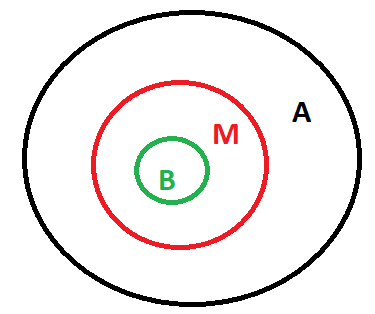
\includegraphics[scale=0.5]{S1DM3.png}

\end{frame}


\begin{frame}
	\titre{Exercices - schémas}

\begin{tabular}{lc}
2$^{\grave{e}me}$ syllogisme & Certains M sont A \\
		& Certains B ne sont pas M \\
\cline{2-2}
		& Certains B ne sont pas A \\
\end{tabular}
\pause

Pas valide : \pause\newline
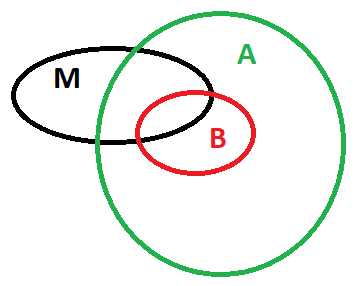
\includegraphics[scale=0.5]{S2DM3.png}

\end{frame}


\begin{frame}
	\titre{Exercices - schémas}

\begin{tabular}{lc}
3$^{\grave{e}me}$ syllogisme & Aucun M n'est A \\
		& Certains B sont M \\
\cline{2-2}
		& Certains B ne sont pas A \\
\end{tabular}
\pause
\textcolor{white}{lol}\newline

Valide : \pause La deuxième prémisse nous dit qu'il existe un individu qui est B et M, qu'on appellera $x$. \pause\newline

Or, la première prémisse nous dit que A et M sont des propriétés incompatibles. $x$, qui est déjà M, ne peut donc pas être A.\pause\newline

On a donc bien un individu, $x$, qui est B mais pas A
\end{frame}


\begin{frame}
	\titre{Exercices - schémas}

\begin{tabular}{lc}
4$^{\grave{e}me}$ syllogisme & Certains M sont A \\
		& Tous les B sont M \\
\cline{2-2}
		& Certains B ne sont pas A \\
\end{tabular}
\pause

Pas valide : \pause\newline
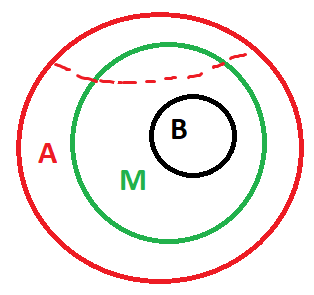
\includegraphics[scale=0.5]{S4DM3.png}

\end{frame}


%	
% \begin{frame}
% \titre{Rappels sur les propositions}
% 
% En linguistique, on dit que P et Q sont \textbf{contradictoires} ssi P et Q ne peuvent être ni vraies, ni fausses en même temps\pause, cad qu'il y en a toujours \textbf{exactement} une des deux qui est vraie\pause\newline
% 	
%Les logiciens, eux, disent que Q est la négation de P (ou l'inverse), et le notent $P \leftrightarrow \neg Q$. \pause On notera parfois (et de plus en plus) $\neg P$ (ou non-P) la proposition contradictoire / négation de P\pause\newline
%
%`non-(Takashi Miike est un réalisateur)` $\equiv$ \pause `Takashi Miike n'est pas réalisateur`\pause\newline
%
%`non-(Takashi Miike est un réalisateur japonais)` $\equiv$ \pause `Takashi Miike n'est pas réalisateur \underline{\textbf{ou}} n'est pas japonais`
% 
% \end{frame}
% 
% 
%\begin{frame}
%	\titre{Rappels sur les propositions}
%	
%
%`non-(P ou Q)` $\equiv$ \pause `(non-P et non-Q)`\newline\pause
%`non-(P et Q)` $\equiv$ \pause`(non-P ou non-Q)` \newline \pause
%
%\textcolor{white}{lalaaa}`non-((P ou Q) et (R ou S))` \newline$\equiv$ \textcolor{white}{lalal}\pause`non-(P ou Q) ou non-(R ou S)` \pause\newline
%$\equiv$ `(non-P et non-Q) ou (non-R et non-S)`\pause \newline
%
%
%\textcolor{white}{lalaaaa}`non-((P et Q) ou (R et S))` \newline$\equiv$ \textcolor{white}{lalaal}\pause`non-(P et Q) et non-(R et S)` \pause\newline
%$\equiv$ `(non-P ou non-Q) et (non-R ou non-S)` \pause \newline
%
%\end{frame}
%
%
%\begin{frame}
%	\titre{Rappels sur les propositions}
%	
%En linguistique, P et Q sont contraires ssi elles ne peuvent pas être vraies en même temps (elles sont incompatibles)\pause\newline
%
%En logique, il n'y a pas - à ma connaissance - de mot ou notation dédié\pause\newline
%
%Proposition\textbf{s} contraire\textbf{s} de `TM est un réalisateur japonais` ?\pause\newline
%
%`TM n'est pas réalisateur` / `TM n'est pas japonais` / `TM n'est ni réalisateur, ni japonais` / `TM n'est pas réalisateur ou n'est pas japonais`
%\end{frame}
%
%
%\begin{frame}
%	\titre{Rappels sur les propositions}
%	
%En linguistique, P et Q sont contraires ssi elles ne peuvent pas être vraies en même temps (elles sont incompatibles)\newline
%
%
%Proposition\textbf{s} contraire\textbf{s} de `TM est un réalisateur japonais` ?\pause\newline
%
%Mais aussi, `TM est réalisateur mais n'est pas japonais` / `TM est japonais mais n'est pas réalisteur` / `TM n'est pas réalisateur et il fait beau et j'ai mal dormi et le numéro gagnat du loto de demain est le 12469820`, etc...\pause Il y a une infinité de props contraires !\pause\newline
%
%On peut voir la proposition contradictoire de P comme sa plus \textit{faible} proposition contraire
%\end{frame}